\begin{abstract}
In this paper the dynamical behavior of systems in states of self-organized criticality is studied using the example
of sandpiles in two and three dimensions. Two distinct models inheriting different characteristics are implemented,
one of them being the Bak-Tang-Wiesenfeld model, the other an independent approach.
The scaling exponents of the three observables \textit{size, duration} and \textit{area} of avalanches are determined
for both models. This is achieved by conducting an analysis of their moments in order to extract the scaling exponents
as well as their uncertainties. Apart from slight deviations in the custom model, due to its different nature,
the results are in good accordance with the literature values obtained from a composition of many distinct authors.
%Slight deviations from the literature occur in the custom model due to its different nature.
%Further deviations for large lattice sizes in three dimensions are due to the limited amount of simulations,
%time and resources.
\end{abstract}

\maketitle

\section{Introduction}
\label{sec:intro}
In this paper we investigate the evolution of sandpiles into states of so-called self-organized criticality (SOC) using
two different models for simulation. Furthermore we analyze the sandpiles' scaling behavior and scaling exponents.

Self-organized criticality describes a special case of the very general concept of criticality. Every system
exhibiting self-organized criticality has in common the occurrence of macroscopic scale invariant properties.
In the picture of a real sandpile this can be seen by looking at the average slope of the sandpile,
which stays constant even if the sandpile is enlarged by adding more and more sand to it.
It is notable that this is the case despite the dynamics of a pile of sand is actually governed by complicated
microscopic\footnote{Microscopic in the sense of the size of a sand grain compared to the whole pile.} interactions
of its many constituents, the sand grains.

Such self-organized criticality has been observed before in simulations of sandpiles carried out by Bak, Tang and
Wiesenfeld in the 1980s. It is indeed interesting to further analyze such a sandpile model
because it can serve as a toy model for many other similar behaving systems like landslides, rock falls, earth quakes
etc., which all follow from different physical processes, though.
In the mentioned systems signs of self-organized criticality have been observed, not only from simulations but also
from real-world data~\cite{Hergarten}.

We simulate the sandpiles using a cellular automaton algorithm analog to the approach of Bak, Tang and Wiesenfeld,
which is commonly referred to as the \enquote{BTW model}. Scaling exponents are determined and compared to the
results of a customized sandpile model.

Section~\ref{sec:theory} starts with an overview on the theory behind self-organized criticality and in particular
explains the scaling behavior governed by the scaling exponents.
In Section~\ref{sec:experiment} our implementation of the sandpile cellular automata is shown as well as
the used methods for extracting the relevant parameters from the generated data.
The results are presented in Section~\ref{sec:results} and discussed in Section~\ref{sec:discussion}.


\section{Theory}
\label{sec:theory}

\subsection{Self-organized criticality}
\label{sec:th:SOC}
To understand the concept of self-organized criticality consider first a system that exhibits a critical state,
like the Ising model. The critical state in the Ising model corresponds to a phase transition where vanishing
magnetization evolves into spontaneous magnetization. This happens at a specific temperature, the critical temperature
$T_{\mathrm{crit}}$. To obtain a system in the critical state, the temperature has to be precisely tuned to the critical
temperature.

The criticality of the system leads to scale invariant properties. For instance clusters of the same spin direction
will form and the size distribution of these clusters follows a simple power law. A power law distribution implies
scale invariance, where scale invariance means that the dynamics of the considered system do not change if the system
is scaled by some global factor. In particular the observables' distribution functions keep the same form.

The crucial difference of this definition of criticality and the criticality observed in the case of the sandpile model
is that sandpiles will evolve into a critical state without tuning of any critical parameter.
If enough sand is deposited into a sandbox or, respectively, enough iteration steps of the computer model are performed
it reaches an equilibrium state by itself with a fixed average slope. This self-organization into a critical state
always happens, independently of the actual detailed model parameters\footnote{Note that the slope can still depend
on these parameters.}. Thus this phenomenon is called \enquote{self-organized criticality}.

\subsection{Scaling exponents}
\label{sec:th:scaling}
If there is scale invariance in a system it can be directly observed in the distribution functions
of the observables of the system as indicated above. Consider some observable $\hat{Y}$ that can be measured in the
present system. If this observable is measured many times and histogrammed one obtains a distribution according to the
corresponding probability density function $P^{Y}(y)$.
If now the system is scaled by a factor $\lambda$ it must hold
\begin{equation}\label{eq:scalingCondition}
P^{Y}(\lambda y) = f(\lambda) \times P^{Y}(y)
\end{equation}
due to the assumed scale invariance.

As scale invariance is suspected as a main property of SOC models in general, one is mainly interested in studying
these distribution functions to test this hypothesis. To do this a theoretical prediction is necessary first.
In the simplest approximation the distribution function of an observable $\hat{Y}$ in a scale invariant SOC model
is assumed to follow a simple power law
\begin{equation}\label{eq:simpleScaling}
P^{Y}(y) \sim y^{-\rho}
\end{equation}
in order to fulfill Equation~\eqref{eq:scalingCondition} as $(\lambda y)^{-\rho}\sim y^{-\rho}$.
Here $\rho$ is called the \emph{critical exponent} of the observable $\hat{Y}$.

However, in a real implementation of the sandpile model or any other SOC model one has to deal with finite system sizes
since infinitely large systems can neither be simulated nor do they exist in nature.
A finite system size limits the validity of Equation~\eqref{eq:simpleScaling} because for instance avalanche sizes on a
sandpile are naturally limited to the size of the sandpile itself. Thus a more sophisticated description of scaling
has to be used, so-called \emph{finite-size scaling} as described in \cite{SOC-book}:
\begin{equation}\label{eq:finiteSizeScaling}
P^{Y}(y) = a y^{-\rho} G^{Y}\left(\sfrac{y}{y_c(L)}\right), \quad y_c(L)=b L^K
\end{equation}
The additional scaling function $G^{Y}$ accounts for limited size corrections to the simple power law scaling
by modifying the probability density for values of $y$ in the order of the limiting \emph{characteristic scale}
$y_c(L)$. This characteristic scale where limitations eventuate can itself depend on the system size $L$,
e.g. the maximum area coverage of a two dimensional lattice is $L^2$. Thus the characteristic scale is approximately
assumed to behave as $y_c(L)=b L^K$ for any observable, where $b,K$ depend on $\hat{Y}$.
The set of the critical exponent $\rho$ together with the \enquote{observable's dimension} $K$ are
generally called finite-size scaling exponents or short scaling exponents.

One possibility to obtain the finite-size scaling exponents $\rho$ and $K$ from the measured distribution functions
is via their moments $\langle y^n\rangle$. These moments follow from Equation~\eqref{eq:finiteSizeScaling} by integration
and as is shown in~\cite{SOC-book} in the limit of an infinitely large lattice this yields
\begin{equation}\label{eq:momentScaling}
\langle y^n\rangle(L) \xrightarrow[L\to\infty]{} a g^{Y}(0) (bL)^{\sigma_n},\quad \sigma_n := K(1+n-\rho),
\end{equation}
with $g^{Y}(0)=\mathrm{const.}$ a definite integral containing the scaling function $G^{Y}$.
Equation~\eqref{eq:momentScaling} is as an approximation also valid for finite but large enough lattice sizes where
the observable's characteristic scale is much larger than a certain lower cutoff parameter. This lower cutoff may arise
from the detailed microscopic interactions and the discreteness of the lattice, i.e. $L \gg 1$ for a lattice divided
into discrete cells of edge length $1$ can in principle yield sufficiently good results.

Using Equation~\eqref{eq:momentScaling} the scaling exponents could now be calculated from any measured distribution
function by doing simple linear regressions to log-log plots of different moments $\langle y^n\rangle (L)$ against $L$.
Combining the parameters $\sigma_n$ from the regression for different $n$ provides $\rho$ and $K$.

\section{Experimental Methods}
\label{sec:experiment}

\subsection{Cellular Automata}
\label{sec:cellularAutomata}
To realize the simulation of sandpiles it is convenient to construct a cellular automaton.
A cellular automaton is an algorithm that takes values on a discrete $n$-dimensional lattice and repeatedly performs
updates on all lattice sites with each updated value only depending on the old value and the values of its nearest
neighbors (and possibly random numbers). Additionally the lattice sites can be periodically perturbed, for instance
increasing the value of a randomly picked lattice site.

\subsection{Implementation of sandpile cellular automata}
\label{sec:sandpileImplementation}
In general a cellular automaton for a sandpile in $\mathcal{N}$ real dimensions works on an $\mathcal{N}-1$ dimensional
lattice where each lattice site stands for a stack of sand grains in the left dimension. That means for example that
a real sandpile, which is three dimensional, is simulated on a two dimensional lattice reflecting the ground as $x$-$y$
plane. The entry on each site then characterizes how many grains of sand are stacked in the $z$ direction.
We will denote these lattice entries by the variable $s(\vec{r})$ in the following, with the discrete lattice sites
$\vec{r}=(x,y,\ldots)^\top$.

It can be either chosen to store the actual amount of grains as the entry $s$ or the slope with respect to the
vicinity of the stack. Both choices enable for sufficient characterization and simulation of the microscopic
dynamics of the sandpile. Choosing the slope entries, however, has the drawback that the model will then be
non-isotropic anymore, as will become clear in the following, whereas storing the actual heights can make the model
implementation a bit more complex.

Within the scope of this paper we have implemented two different cellular automata that are based on these two different
choices.

\subsubsection{The BTW model}
The first approach reflects the BTW model. The BTW model by Bak, Tang and Wiesenfeld~\cite{BakTangWiesenfeld:1987}
is the first model investigating SOC in sandpile dynamics. It uses a lattice that contains slope values and
alternatingly performs a \emph{driving} and a \emph{relaxation} of the lattice:

\textbf{Driving} generally describes the active perturbation of the lattice. For a real sandpile the perturbation
intuitively consists of adding a grain of sand to the pile at a random position. Since the BTW model deals with
slopes the addition of one grain of sand could not be achieved by just increasing $s(x,y)$ about one but the neighboring
entries would have to be changed, too. This type of driving is called \emph{conservative driving}
(see Figure~\ref{fig:driving:cons}).
For the BTW model, however, we decided to use \emph{non-conservative driving} described by simply adding one slope
unit to the considered lattice site:
\begin{itemize}
\item $s(\vec{r}) \mapsto s(\vec{r})+1$
\end{itemize}
The non-conservative driving can be thought of as adding grains of sand to \emph{all} uphill sites with respect to
$\vec{r}$ (Figure~\ref{fig:driving:non-cons}), which is of course unphysical but converges much faster to the
SOC state~\cite{Christensen1991}. It can still reproduce results similar to the conservative algorithm when the same,
physical, relaxation algorithm is used.

\begin{figure}[htb]
    \centering
    \begin{subfigure}{0.48\linewidth}
        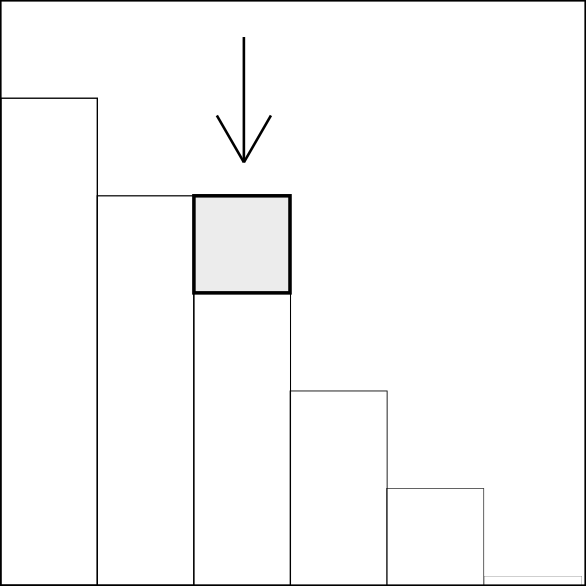
\includegraphics[width=0.85\linewidth]{drivingCons}
        \caption{Conservative driving.}
        \label{fig:driving:cons}
    \end{subfigure}
    \begin{subfigure}{0.48\linewidth}
        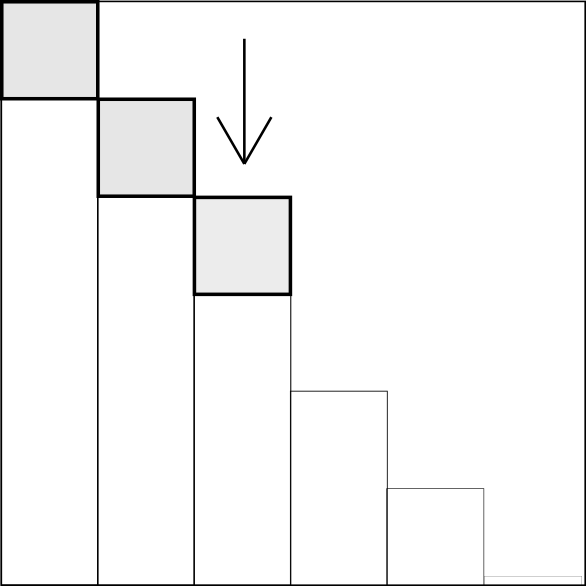
\includegraphics[width=0.85\linewidth]{drivingNonCons}
        \caption{Non-conservative driving.}
        \label{fig:driving:non-cons}
    \end{subfigure}
    \caption{Driving of a one dimensional sandpile where the columns in the sketch display
             the \emph{actual pile heights}.}
    \label{fig:driving}
\end{figure}

\textbf{Relaxation} takes place after a driving step has performed. If the sandpile becomes too steep somewhere on the
lattice, i.e. $s \geq s_{\mathrm{crit}}$ with the \emph{critical slope} $s_{\mathrm{crit}}$, after sand has been added
the pile gets instable. It locally collapses and thus creates avalanches of sand sliding down the pile until the slope
recovers to a non-critical value again. In the BTW model the critical slope is usually fixed to
$s_{\mathrm{crit}}=2\times\operatorname{Dim}\left[\vec{r}\right]$. For each site with critical slope the following
relaxation algorithm is performed:
\begin{itemize}
\item $s(\vec{r}) \mapsto s(\vec{r}) - 2\times\operatorname{Dim}\left[\vec{r}\right]$
\item $s(\vec{r}\pm\vec{\mathrm{e}}_i) \mapsto s(\vec{r}\pm\vec{\mathrm{e}}_i) + 1,
\quad \forall i\in[1,\operatorname{Dim}\left[\vec{r}\right]]$
\end{itemize}
If after the relaxation any site is still critical or if any other site has become critical in the process of
relaxation the relaxation procedure is repeated until there is no critical site on the lattice anymore.
Every repetition of the relaxation procedure counts as one unit time step.

To translate this relaxation routine to the picture of a real sandpile it calculates the local slope of the sandpile as
the sum of the local slope (= stack height difference) in $x$-direction and the local slope in $y$-direction.
If this summed slope reaches the critical slope value $s_{\mathrm{crit}}$, for each dimension one grain of sand is
redistributed from the site to its downhill nearest neighbors. This results in a consistent description of a lattice
containing slopes and the two procedures for driving and relaxation.

The fact that the slopes $s$ are only integer numbers naturally implies that they cannot contain any information about
the direction of the slope. If one takes the real sandpile picture from above into account again it becomes clear that
the slope direction is fixed to the same diagonal for every lattice point. This is an inherent feature of the BTW model
as a result of the reduction to storing slopes instead of stack heights. It creates a preferred direction for avalanches
and thus makes the model \emph{non-isotropic} such that the BTW critical state must be principally thought of as a
\enquote{diagonal hillside}.

\subsubsection{The custom model}
The second approach for the sandpile simulations uses the local height or number of sand grains as lattice entries.
Thus it can circumvent the problem of the BTW model to be non-isotropic because the slopes can be directly calculated
from the heights in every direction.
The overall implementation of the custom model cellular automaton essentially follows the implementation of BTW model.
Since in the custom model the lattice entries $s(\vec{r})$ are heights instead of slopes the relaxation procedure
works differently compared to the BTW model, though.
For the slope between two neighboring sites $\vec{r}_1$ and $\vec{r}_2$ the difference $s(\vec{r}_1)-s(\vec{r}_2)$ is
used. If the absolute value of this slope reaches the critical value $q_{\mathrm{crit}}$ the site with the higher
stack is called critical site. The critical slope $q_{\mathrm{crit}}$ is a free parameter in this custom model.

If now one site is critical with respect to at least one of its nearest neighbors the stack is considered unstable
and about to collapse. All excess sand grains with respect to the neighbor with the least height will then be
redistributed to all nearest neighbors to which the slope is at least critical until none of slopes to the neighbors
is critical anymore. This represents one unit time step.
Since grains have been redistributed and slopes could have changed, in the next relaxation step all nearest neighbors
of the critical site are checked if they have become critical. Like in the BTW model this is repeated until no site
is critical anymore and the avalanche stops.

The driving procedure simply consists of increasing $s(\vec{r})$ about $1$.

In the custom model it is possible to choose different boundary conditions for each edge of the lattice independently.
It can be chosen between \emph{open} and \emph{closed} boundary conditions. The closed boundaries basically model an
infinitely high wall that does not let any sand grains pass whereas the open boundaries can be thought of as the edge
of a table where any excess sand can just drop from the table. This means that sand grains can fall of the lattice at
open boundaries but accumulate at closed boundaries.
In order to make the comparison of the BTW model and the custom model possible the configuration of
$\operatorname{Dim}\left[\vec{r}\right]$ neighboring open boundaries meeting at one corner of the lattice and
respectively $\operatorname{Dim}\left[\vec{r}\right]$ neighboring closed boundaries was chosen for the simulations,
which yields a \enquote{diagonal hillside} for the custom model, too.

\subsection{Extraction of scaling exponents}
\label{sec:extractCritExp}
Since we want to study the SOC scaling behavior of sandpile avalanches we need to extract scaling exponents of
different observables. Besides the two most intuitive observables that characterize an avalanche, the \emph{area},
the \emph{time duration} and the \emph{linear size}/\emph{radius}, there is another quantity that is typically considered
in SOC studies, which is slightly misleadingly called \emph{size} of an avalanche. The size quasi describes the overall
instability released in the avalanche or also the total mass-, momentum- or energy dissipation of the avalanche.
For the automaton algorithms we precisely define all four observables as follows:
\begin{description}
\item[Size] The number of critical sites accumulated over all repetitions of the relaxation procedure.
\item[Duration] The number of unit time steps from the triggering of the avalanche until it stops. The unit time step
                corresponds to one repetition of the relaxation routine.
\item[Area] The $\operatorname{Dim}\left[\vec{r}\right]$ dimensional volume that contains the avalanche,
            i.e. the number of lattice sites that took part in the avalanche.
\item[Linear size] The maximum (euclidean) distance between any pair of sites that took part in the avalanche.
\end{description}
The calculation of the linear size gets very computing-intensive and memory consuming for large
lattice sizes $L$ and has thus been disabled during our full simulations. In this paper we concentrate
on investigating the size, duration and area.

To each of the three considered observables needs to be assigned a set of scaling exponents $(\rho,K)$
according to Equation~\eqref{eq:finiteSizeScaling}:
\begin{description}
\item[Size] critical exponent $\tau$, avalanche dimension $D$.
\item[Duration] critical exponent $\alpha$, dynamical exponent $Z$.
\item[Area] critical exponent $\kappa$, avalanche area dimension $T$.
\end{description}

As pointed out in Section~\ref{sec:th:scaling} the exponents can be determined from the corresponding measured
distributions. To obtain these distributions one full simulation run needs to be performed, which alternatingly performs
a driving and triggering of a relaxation of the lattice as described in Section~\ref{sec:sandpileImplementation}.
This happens until a certain given number of drives is reached. Each relaxation between two drives corresponds to an
avalanche\footnote{Here we count no triggered avalanches as zero-size avalanches}. The desired observables are
calculated within the relaxation procedure for each avalanche and the values for all avalanches are in the end stored
by the main program. The stored data then represent samples of the underlying distribution functions.

Given a sample of one of these distributions, the distribution's first and second moment is estimated via
\begin{equation}
\langle y^n\rangle(L) := \int\!\mathrm{d}y\, y^n P^{Y}(y) \simeq \sum_i y_i^n \Big/ \sum_i y_i^0,\quad n=1,2,
\end{equation}
where $L$ is the lattice size used in the simulation and $y_i$ the measured value of $\hat{Y}$ in the $i$-th avalanche.
According to Section~\ref{sec:th:scaling} we plot $\ln\left(\langle y^n\rangle(L)\right)$ against $\ln\left(L\right)$
using simulations for different values of $L$ and apply a linear regression to the plot. This yields a straight line
with slope $\sigma_n$, such that $\rho, K$ follow from:
\begin{equation}
\rho = \frac{2\sigma_2 - 3\sigma_1}{\sigma_2 - \sigma_1}, \qquad\qquad K = (\sigma_2-\sigma_1)
\end{equation}

To enable for estimating uncertainties via bootstrapping, each simulation run must be applied multiple times such that
multiple samples of the distribution lead to multiple measurement values of $\ln\left(\langle y^n\rangle(L)\right)$
for constant $L$. We use a double bootstrap procedure in order to do a complete linear regression
including the covariance matrix of the measurement points
$\langle\ln\left(\langle y^n\rangle(L_i)\right), \ln\left(\langle y^n\rangle(L_j)\right)\rangle$.


\section{Simulation Results}
\label{sec:results}
To achieve sufficiently good statistics also for the larger, i.e. rarer, avalanches each simulation was set up to
do $100000$ random drives and was repeated ten times for doing the bootstrap. Simulations were done for both models
in two and three dimensions for lattice sizes ranging from \SIrange{10}{100}{}.

All the sandpile lattices used for the simulations have been filled and driven to a self-organized critical state
beforehand using the same two cellular automata. For this purpose these were kept running until the averaged slope of
the piles did not change significantly anymore, measured across a certain amount of drives in between.

\subsubsection{BTW model}
In Figure~\ref{fig:btwSandbox} one exemplary two-dimensional critical sandbox for the BTW model is shown,
which represents one of the sandboxes that were used as initial sandbox for the later simulations.
\begin{figure}[htb]
    \centering
    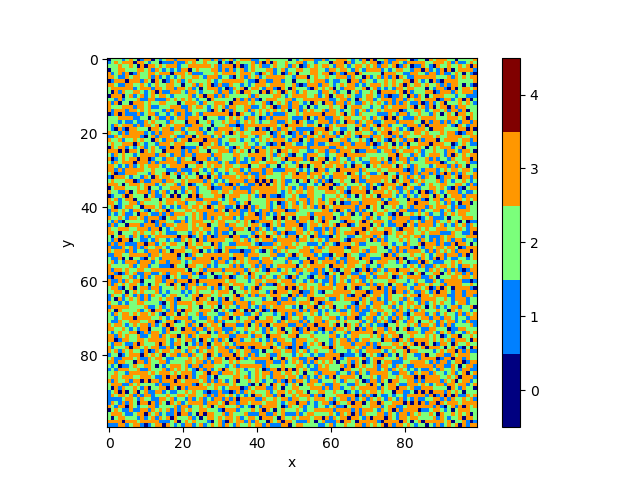
\includegraphics[width=\linewidth]{plots/sandboxes/BTW_100x100}
    \caption{Critical two-dimensional sandbox of the BTW model with lattice size $L=100$.}
    \label{fig:btwSandbox}
\end{figure}

Avalanches of different size and shape occurred in the simulations. Figure~\ref{fig:btw2DAvalanche} shows one example
of the avalanches recorded for a two-dimensional sandbox.
\begin{figure}[htb]
    \centering
    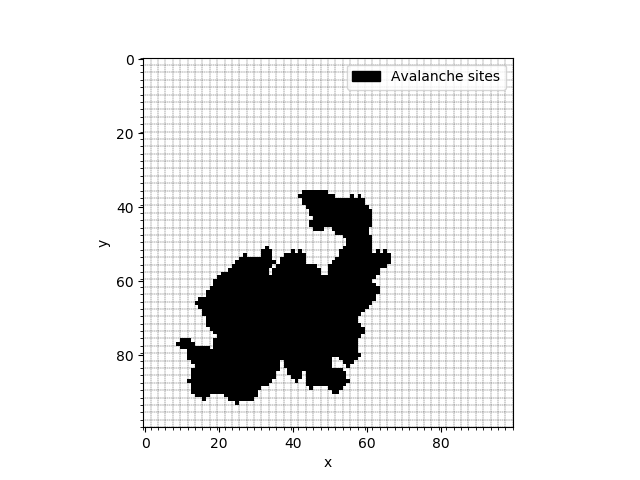
\includegraphics[width=\linewidth]{avalanches/Avalanche_2d_btw_1_report}
    \caption{Avalanche of the BTW model in a two-dimensional sandbox with lattice size $L=100$.
             Every black entry stands for a site that took part in the avalanche by relaxing
             at least once during the whole avalanche.}
    \label{fig:btw2DAvalanche}
\end{figure}

In Figure~\ref{fig:btwSizeFit} the bootstrapped linear regression of the first and second moment of the avalanche size
distribution is shown for a two-dimensional sandbox. The data show only minor deviation from the straight line fit.
The fits for avalanche area and duration yield similar results, also for three-dimensional lattices.
The resulting scaling exponents for two- and three-dimensional lattices are written down in the summarizing
Table~\ref{tab:scalingExp} on page \pageref{tab:scalingExp}.
\begin{figure}[htb]
    \centering
    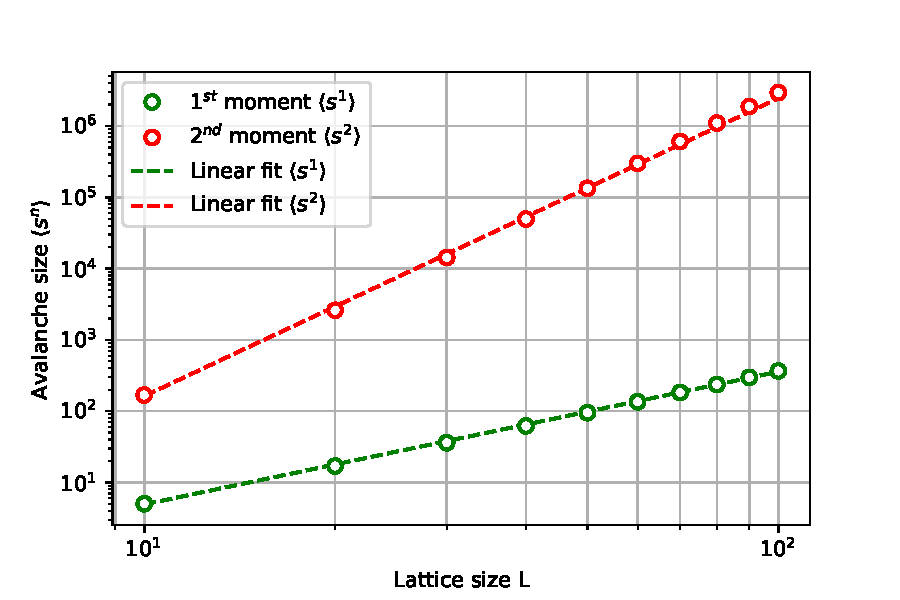
\includegraphics[width=\linewidth]{moment_analysis_size_2d_btw_fit_report}
    \caption{Log-log plot of the first and second moments of the avalanche size distribution of two-dimensional
             sandboxes (BTW model) against $L$ including bootstrapped straight line fits.
             The displayed data points are mean values over ten repeated simulations.
             Error bars are too small to be visible.}
    \label{fig:btwSizeFit}
\end{figure}

\subsubsection{Custom model}
Figure~\ref{fig:customSandbox} shows a sandbox obtained from the custom model simulations with $q_{\mathrm{crit}}=7$,
open boundary conditions at the bottom and left edge and closed boundary conditions at the top and right edge.
\begin{figure}[htb]
    \centering
    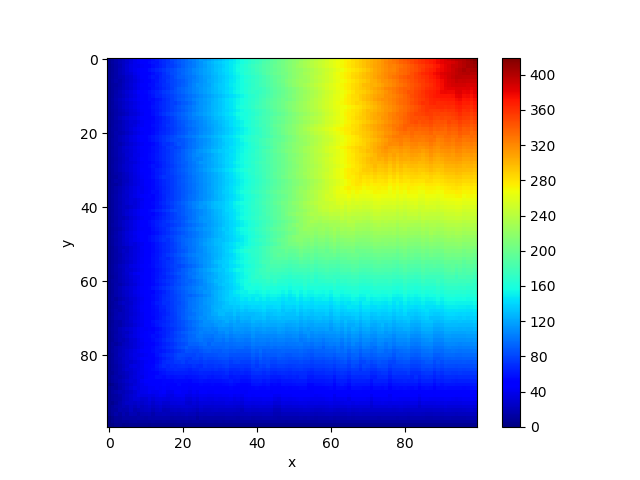
\includegraphics[width=\linewidth]{sandboxes/CST_100x100_cs7}
    \caption{Critical two-dimensional sandbox of the custom model with lattice size $L=100$ and
             critical slope $q_{\mathrm{crit}}=7$.
             The boundary conditions are open at the bottom and left edge and closed otherwise.}
    \label{fig:customSandbox}
\end{figure}

Note again that this sandbox displays heights and not slopes and hence looks completely different than the BTW sandbox
in Figure~\ref{fig:btwSandbox}. To roughly compare both sandboxes one can have a look at Figure~\ref{fig:cstSlopebox},
which shows how this sandbox would appear in the BTW model, i.e. shows the corresponding BTW-like slopes, which are
a superposition of the slopes in $x$- and $y$-direction.
\begin{figure}[htb]
    \centering
    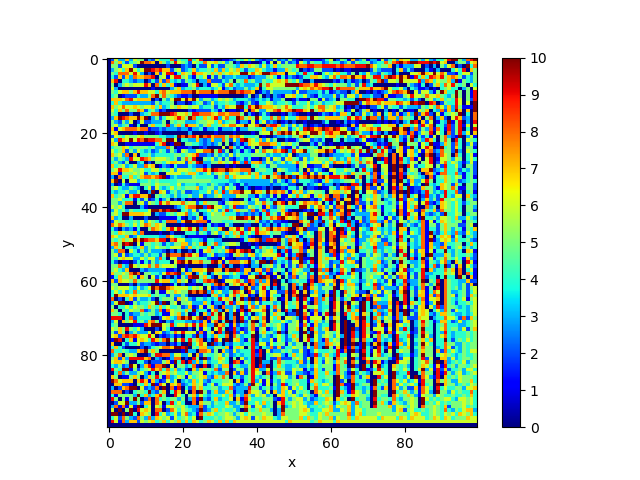
\includegraphics[width=\linewidth]{sandboxes/CST_100x100_cs7_slopeBox}
    \caption{Critical custom model sandbox from Fig.~\ref{fig:customSandbox} that has been transformed from heights to
             BTW-compatible summed slopes. Traces of recent avalanches are clearly visible.}
    \label{fig:cstSlopebox}
\end{figure}

The avalanches observed in the custom model simulations are typically smaller and of a more elongated shape compared
to the avalanches of the BTW model. Figure~\ref{fig:custom2DAvalanche} shows one example of the avalanches recorded
for a two-dimensional sandbox.
\begin{figure}[htb]
    \centering
    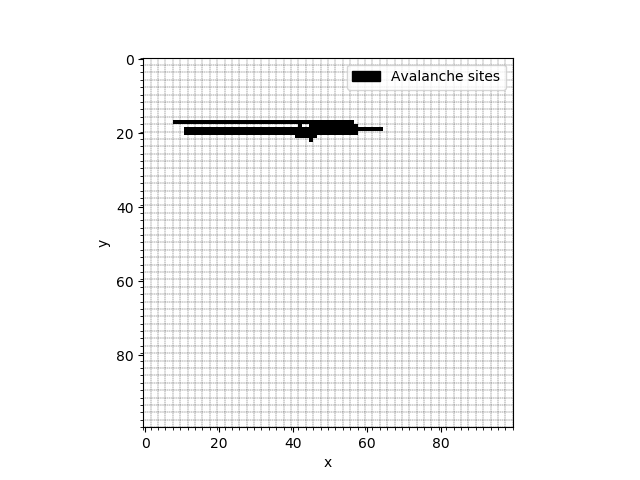
\includegraphics[width=\linewidth]{avalanches/Avalanche_2d_custom_6_report}
    \caption{Avalanche of the custom model in a two-dimensional sandbox with lattice size $L=100$.}
    \label{fig:custom2DAvalanche}
\end{figure}
Traces of the most recent of these avalanches can be even seen in the sandbox itself (Figure~\ref{fig:customSandbox}).

Analog to the case of the BTW model we show the linear fits of the first and second moment of the avalanche size
distribution for a two-dimensional sandbox in Figure~\ref{fig:customSizeFit}.
The straight lines do not fit to the data as good as the ones for the BTW model but for different runs of the
bootstrap fitting the slope and fit quality changed noticeable. This seems to be caused by the limited amount of only
ten measurements per lattice size $L$, which might not represent an ideal base sample for the bootstrap.
The figure shows the fit run that yielded the smallest error on the resulting exponents.
\begin{figure}[htb]
    \centering
    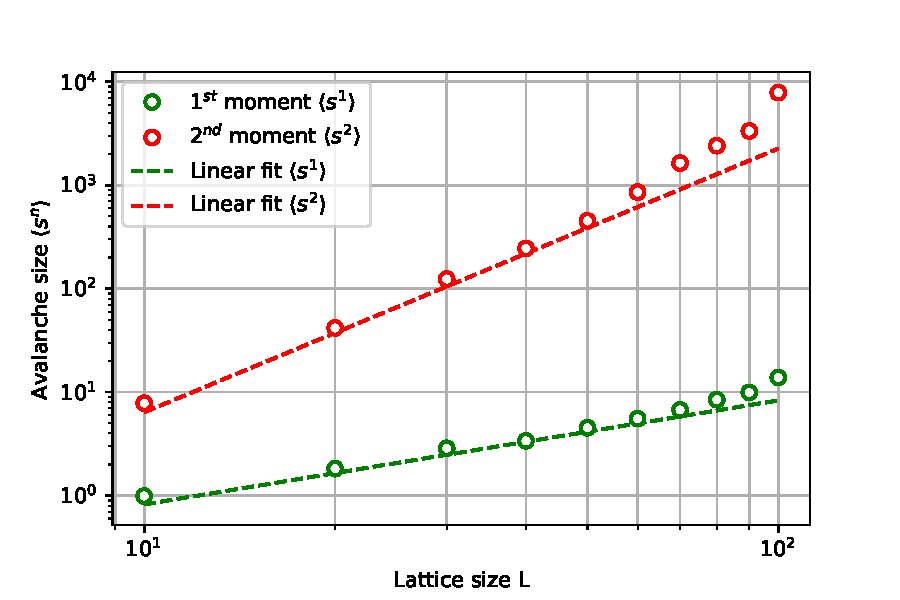
\includegraphics[width=\linewidth]{moment_analysis_size_2d_custom_crit_slope_7_fit_report}
    \caption{Log-log plot of the first and second moments of the avalanche size distribution of two-dimensional
             sandboxes (custom model) against $L$ including bootstrapped straight line fits.
             The displayed data points are mean values over ten repeated simulations.
             Error bars have been omitted for reasons of clarity.}
    \label{fig:customSizeFit}
\end{figure}

The resulting scaling exponents for two- and three-dimensional lattices are summarized in Table~\ref{tab:scalingExp}
together with the results for the BTW model. Results for different values of the critical slope parameter of the
custom model are given.
%
\renewcommand{\arraystretch}{1.5}
\begin{table}[htb]
    \centering
    \caption{Scaling exponents for avalanche size, duration and area for two- and three-dimensional (2D/3D)
             simulations of the BTW model (BTW) and the custom model (CST). The free parameter critical slope
             $q_{\mathrm{crit}}$ of the custom model is denoted by the index C\,$q_{\mathrm{crit}}$.}
    \begin{minipage}{\linewidth}
    \begin{tabular}{lSScSScSSr}
    \toprule
    \multirow{2}{*}{Model} & \multicolumn{2}{c}{Size} && \multicolumn{2}{c}{Duration} && \multicolumn{2}{c}{Area} & \\
    \cmidrule{2-3} \cmidrule{5-6} \cmidrule{8-9}
    & {$\tau$} & {$D$} && {$\alpha$} & {$Z$} && {$\kappa$} & {$T$} & \\
    \midrule
    \midrule
    $\mathrm{BTW}$ & 1.19(9) & 2.3(2) && 1.21(2) & 1.34(3) && 1.23(7) & 1.9(2) &
        \hspace{-20px}\rdelim\rbrace{3}{0mm}[$2$D] \\
    $\mathrm{CST}_{\mathrm{C}5}$ & 1.3(2) & 1.6(2) && 1.2(2) & 0.7(2) && 1.3(2) & 0.8(2) & \\
    $\mathrm{CST}_{\mathrm{C}7}$ & 1.4(2) & 1.6(4) && 1.3(1) & 0.81(8) && 1.4(1) & 1.0(1) & \\
    \midrule
    $\mathrm{BTW}$ & 1.3(1) & 2.5(3) && 1.45(3) & 1.41(6) && 1.4(3) & 2.6(7) &
        \hspace{-20px}\rdelim\rbrace{2}{0mm}[$3$D] \\
    $\mathrm{CST}_{\mathrm{C}5}$\footnote{Values only based on simulations for lattice sizes $10,20,30,40$ due to
                                          limited computational resources. Hence bootstrapped fitting failed and
                                          external fit library was used.}
                   & 1.23(1) & 1.99(2) && 1.29(1) & 1.17(1) && 1.29(1) & 1.43(1)\vspace{2px} & \\
    \bottomrule
    \end{tabular}
    \end{minipage}
    \label{tab:scalingExp}
\end{table}
%--- depending on in which column the table appears use braces on the left- or right-hand side ---
%\begin{table}[htb]
%    \centering
%    \caption{Scaling exponents for avalanche size, duration and area for two- and three-dimensional (2D/3D)
%             simulations of the BTW model (BTW) and the custom model (CST). The free parameter critical slope
%             $q_{\mathrm{crit}}$ of the custom model is denoted by the index C\,$q_{\mathrm{crit}}$.}
%    \begin{minipage}{\linewidth}
%    \begin{tabular}{llSScSScSS}
%    \toprule
%    & \multirow{2}{*}{Model} & \multicolumn{2}{c}{Size} && \multicolumn{2}{c}{Duration} && \multicolumn{2}{c}{Area} \\
%    \cmidrule{3-4} \cmidrule{6-7} \cmidrule{9-10}
%    && {$\tau$} & {$D$} && {$\alpha$} & {$Z$} && {$\kappa$} & {$T$} \\
%    \midrule
%    \midrule
%    \hspace{-20px}\ldelim\lbrace{3}{0mm}[$2$D] &
%      $\mathrm{BTW}$ & 1.19(9) & 2.3(2) && 1.21(2) & 1.34(3) && 1.23(7) & 1.9(2) \\
%    & $\mathrm{CST}_{\mathrm{C}5}$ & 1.3(2) & 1.6(2) && 1.2(2) & 0.7(2) && 1.3(2) & 0.8(2) \\
%    & $\mathrm{CST}_{\mathrm{C}7}$ & 1.4(2) & 1.6(4) && 1.3(1) & 0.81(8) && 1.4(1) & 1.0(1) \\
%    \midrule
%    \hspace{-20px}\ldelim\lbrace{2}{0mm}[$3$D] &
%      $\mathrm{BTW}$ & 1.3(1) & 2.5(3) && 1.45(3) & 1.41(6) && 1.4(3) & 2.6(7) \\
%    & $\mathrm{CST}_{\mathrm{C}5}$\footnote{Values only based on simulations for lattice sizes $10,20,30,40$ due to
%                                            limited computational resources. Hence bootstrapped fitting failed and
%                                            external fit library was used.}
%                   & 1.23(1) & 1.99(2) && 1.29(1) & 1.17(1) && 1.29(1) & 1.43(1)\vspace{2px} \\
%    \bottomrule
%    \end{tabular}
%    \end{minipage}
%    \label{tab:scalingExp}
%\end{table}


\section{Discussion}
\label{sec:discussion}

The sandboxes of both models clearly self-organized into some equilibrium state with temporally constant average slope
and overall appearance. The extraction of scaling exponents based on the finite-size scaling assumption
(Equation~\eqref{eq:finiteSizeScaling}) was possible and even naive power law fits to the histogrammed distributions
indicate scale invariance (see Appendix~\ref{app:naiveFit}).
This confirms the occurrence of SOC in the BTW model as already previosly observed by many other researches
and it shows that SOC also appears in our custom sandpile model.

A SOC state seems to develop in the custom model independently of the value of the critical slope parameter.
Since we only simulated for $q_{\mathrm{crit}}=5$ and $q_{\mathrm{crit}}=7$ we suggest, however, to check this
again for a much broader range of critical slopes.

The avalanches look quite different for the different models. The BTW avalanches appear much more spread over the
lattice than the custom model ones. As one can see in Figure~\ref{fig:customSandbox} the choice of boundary conditions
in the custom model did not completely yield the desired \enquote{diagonal hillside} but rather two split off hillsides
towards the $x$- and $y$-axes. We believe that a further modification of the custom model, namely to allow for dropping
grains to the diagonal nearest neighbors, would yield improved results.
This would also describe the physics more accurate.

There were virtually no large avalanches observed for the three-dimensional custom model. This is possibly due to a
too small critical slope as we have only simulated for $q_{\mathrm{crit}}=5$ in three dimensions due to limited
computational resources.
The critical slope in the BTW model is the fixed parameter of $s_{\mathrm{crit}}=2\times\operatorname{Dim}
\left[\vec{r}\right]$ and is thus automatically increased for larger dimensions.
Simulations in three dimensions with $q_{\mathrm{crit}}\gg 5$ are advisable to achieve improved results.

The bootstrap fits for the extraction of the scaling exponents turned out to be not always reliable. Multiple calls
of the fit routine yielded varying fit qualities and varying scaling exponents so we decided to take the best quality
fits with the smallest errors on the scaling epxonents out of many fit runs. However, the errors are still somewhat
large and we suggest to increase the number of simulation samples for each moment $\langle y^n\rangle(L)$ to a value
considerably larger than only ten.

We obtained particularly bad fitting to the measurement points for the three-dimensional BTW model at large lattice
sizes (see Appendix~\ref{app:btwSizeFit3D}). It is yet unclear if the scaling breaks down at large lattice sizes or
if the \num{100000} drives were just too few drives compared to the number of lattice entries equal to $L^3$.
We suspect that this could be resolved by increasing the number of drives to the order of \num{1000000}.
But care must be taken here since the simulations with less drives and less runs can already take several hours
for each lattice size.

Large lattice sizes in three dimensions for the custom model could not be investigated due to limited computational
resources.

The results for the scaling exponents (see Table~\ref{tab:scalingExp}) of the BTW model can be compared to many
different literature values from various papers~\cite{SOC-book}, which are essentially in accordance with our
measurements for the two-dimensional case. For the three-dimensional measurements we observe slight deviations to
smaller values compared to the literature. It is not always given an appropriate measurement uncertainty in the
literature, though, and also values from different papers are not necessarily compatible to each other
within the uncertainties. Thus we believe that an overall good agreement to the literature is given in two as well as
in three dimensions. Note also that we suppose that too few drives were performed for the three-dimensional
lattices as pointed out before.

The scaling exponents of the custom model are compared to our results of the BTW model to investigate if the different
approaches of scalar slopes vs. heights yield a similar scaling behavior, which we would expect because both models
are supposed to simulate the same system. We still don't necessarily expect exactly matching values due to the
non-isotropic relaxation in the BTW model whereas in the custom model the sand grains are redistributed in a more
isotropic way.

From Table~\ref{tab:scalingExp} one finds the tendency to smaller $K$. Most notably the value for the avalanche area
dimension is about \num{2} in the BTW model and about \num{1} in the custom model. This corresponds to the other,
visual observations of narrow, less spreading avalanches of the custom model.
The avalanche area dimension indeed seems to reflect the dimensionality of the avalanches.
We suggest again to try out incorporating of dropping to the diagonal nearest neighbors to see if it impacts these
observations.

The values for $\rho$ tend to be a bit larger, which would mean a slight suppression of large avalanches compared to
the BTW model, but they are actually compatible with the BTW values within the uncertainties. To resolve this the
uncertainties have to be narrowed down by increasing the number of drives and simulation samples as described above.

All scaling exponents are independent of the chosen critical slope within uncertainties. This should be checked again
with improved resolution, too, as well as it should be checked with a broader range of critical slopes.
In three dimensions we have only simulations for lattice sizes of $L=10,20,30,40$ available due to limited computational
resources. Also the bootstrapped fitting could not be reliably applied such that the values of the three-dimensional
custom model exponents cannot really be considered reliable.


\section{Conclusion}
\label{sec:conclusion}

In this project two different approaches of cellular automata for sandpile dynamics have been implemented and their
dynamic properties investigated. The phenomenon of self-organized criticality and the corresponding scale invariance
of the dynamics were observed for simulations in two and three dimensions for both models which supports the general
concept of scale invariance in self-organized critical systems. With regard to the rather frequently studied
Bak-Tang-Wiesenfeld model, our resulting sets of scaling exponents for avalanche \textit{size} and \textit{duration}
mostly reside within a wide spread of many different reference values corresponding to various authors over several
decades. Some of these references are displayed in \ref{tab:scalingExpLit}. Much less frequently, the exponents of the
avalanche \textit{area} $\kappa,\ T$ are stated in literature which limits the references to only values for $\kappa$.
For 3 dimensions a general deviation to smaller values is most likely due to the insufficient amount of drives for
lattice sizes $L\ge 50$ where the number of drives was smaller than the total sites in the lattice.
Due to the lack of errors on some of the literature values, we are not able to verify exact accordance, though,
the deviations in two dimensions are generally within one $\sigma$. By conducting a moment analysis rather than a
simple linear regression to the PDF of the respective observable, we were able to extract the scaling exponents while
giving a reasonable estimation on their uncertainty as well as taking the influence of the finite size of the lattice
on the PDF (\textit{finite-size effects}) into account. Here, we want to point out that a number greater than ten
simulation samples per lattice size is very likely to improve the moment analysis and ten should be regarded as a lower
limit rather than a desired value. Generally, an increase of samples, drives, lattice sizes and finally dimensions for
both models is likely to improve to the obtained results and narrow down the uncertainties.


\appendix*

\section{}
\label{sec:app}

\subsection{Simple histogrammed power law scaling}
\label{app:naiveFit}
\begin{figure}[!h]
    \centering
    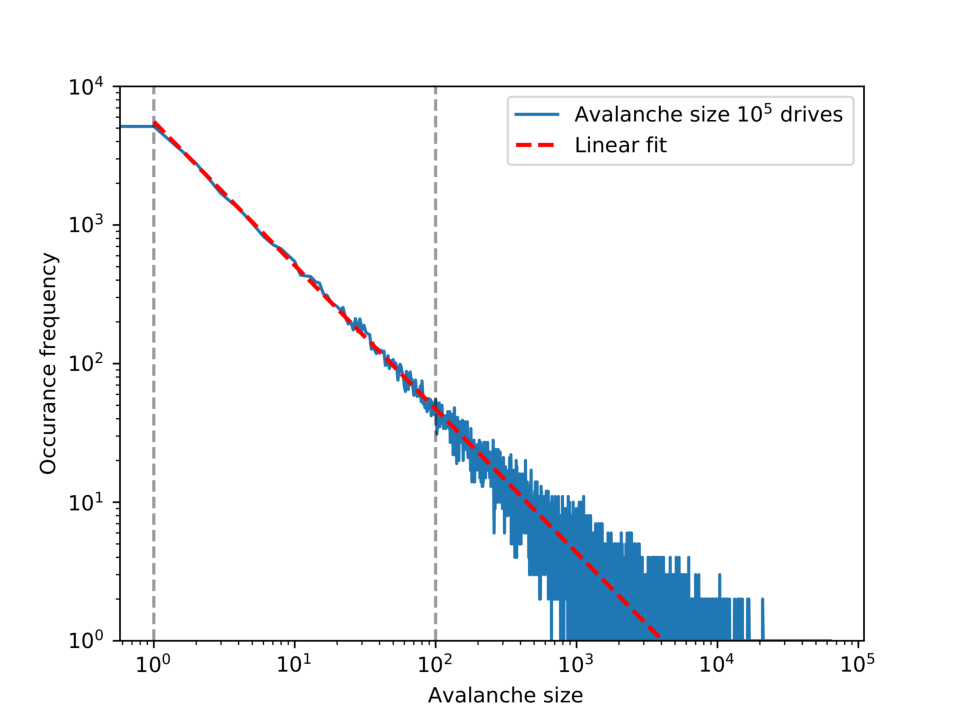
\includegraphics[width=\linewidth]{naive_fits/naive_fit2_report}
    \caption{Naive straight line fit to the raw log-log plot of the avalanche size distribution
             (BTW model, $100\times 100$ lattice) for obtaining the critical exponent $\tau$.}
    \label{fig:naiveFit}
\end{figure}

\subsection{Moment fitting in three dimensions (BTW)}
\label{app:btwSizeFit3D}
\begin{figure}[!h]
    \centering
    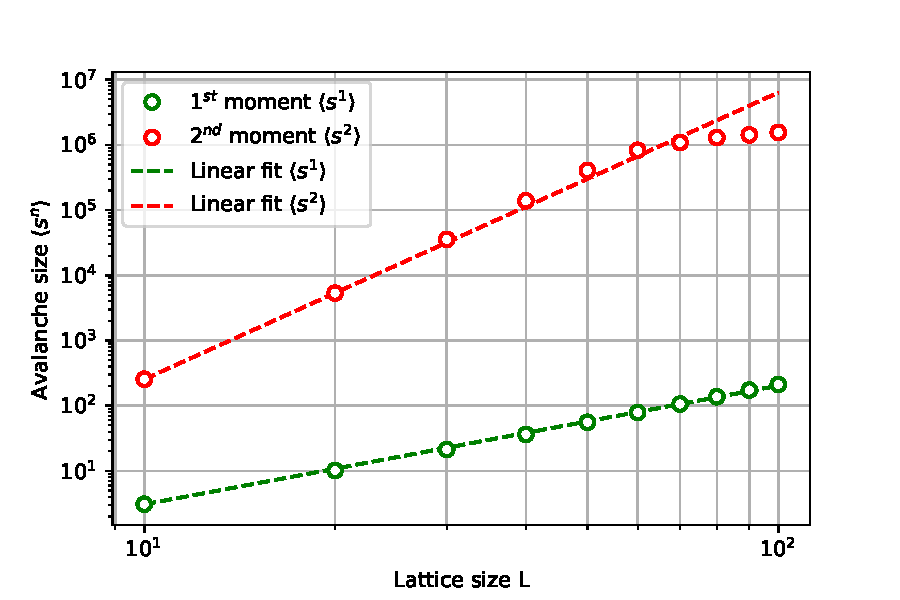
\includegraphics[width=\linewidth]{moment_analysis_size_3d_btw_fit_report}
    \caption{Fitting of first and second avalanche size moments for a three-dimensional sandbox (BTW model).
             The second moments show noticeable deviations from the straight line fit for large lattice sizes.
             Error bars have been omitted for reasons of clarity.}
    \label{fig:btwSizeFit3D}
\end{figure}

\subsection{Literature values of scaling exponents}
\label{app:scalingExpLit}
\renewcommand{\arraystretch}{1.5}
\sisetup{input-decimal-markers={.},output-decimal-marker={.},group-separator={},scientific-notation=fixed,
         fixed-exponent=0,separate-uncertainty=false,table-format=4.4}
\begin{table}[htb]
    \centering
    \caption{Example literature values of scaling exponents for avalanche size and duration
             of the two- and three-dimensional BTW model, taken over from~\cite{SOC-book}.}
    \begin{minipage}{\linewidth}
    \begin{tabular}{lcSScSScSS}
    \toprule
    \multirow{2}{*}{Dim.} && \multicolumn{2}{c}{Size} && \multicolumn{2}{c}{Duration} && \multicolumn{2}{c}{Area} \\
    \cmidrule{3-4} \cmidrule{6-7} \cmidrule{9-10}
    && {$\tau$} & {$D$} && {$\alpha$} & {$Z$} && {$\kappa$} & \\
    \midrule
    \midrule
    $\mathrm{2D}$ && 1.27(1)\,\footnotesize\cite{socbook-ref--k} & 2.73(2)\,\footnotesize\cite{socbook-ref--k} &&
                     1.16(3)\,\footnotesize\cite{socbook-ref--n} & 1.02(5)\,\footnotesize\cite{socbook-ref--q} &&
                     1.333\,\footnotesize\cite{socbook-ref--s} \\
    \midrule
    $\mathrm{3D}$ && 1.333\,\footnotesize\cite{socbook-ref--s} & 3.004\,\footnotesize\cite{socbook-ref--t} &&
                     1.6\,\footnotesize\cite{socbook-ref--s} & 1.618\,\footnotesize\cite{socbook-ref--t} &&
                     1.333\,\footnotesize\cite{socbook-ref--s}\\
    \bottomrule
    \end{tabular}
    \end{minipage}
    \label{tab:scalingExpLit}
\end{table}
